% Chapter Template

\chapter{Results} % Main chapter title

\label{chap:results} % Change X to a consecutive number; for referencing this chapter elsewhere, use \ref{ChapterX}
The solar wind speed data is taken from the instrument Ulysses SWOOPS (todo: Quelle)\\
$v_{sw}$ is assumed to stream only radial for this work.\\
\textbf{Steps vsw} \\ \\
Ich hab jetzt ein Set von v-Komponenten pro PHA-Event. Daraus kann ich berechnen:
(mit: In Komponenten aufgeteilt kann man jetzt Geschwindigkeit im SW-frame berechnen, indem man vsw in R-Richtung abzieht)
\begin{itemize}
	\item Betrag im SW frame
	\item Winkel im w-space (SW frame)
\end{itemize}
B-Feld. Von welchem Instrument? auch RTN-System. Genauso Winkel berechnet.\\
1-min-Mittel (Gyroradius Zeit zeigen) und entsprechend EpQ-Steps den PHAs zugeordnet.
\subsection{Slices}
\begin{figure}[h]
	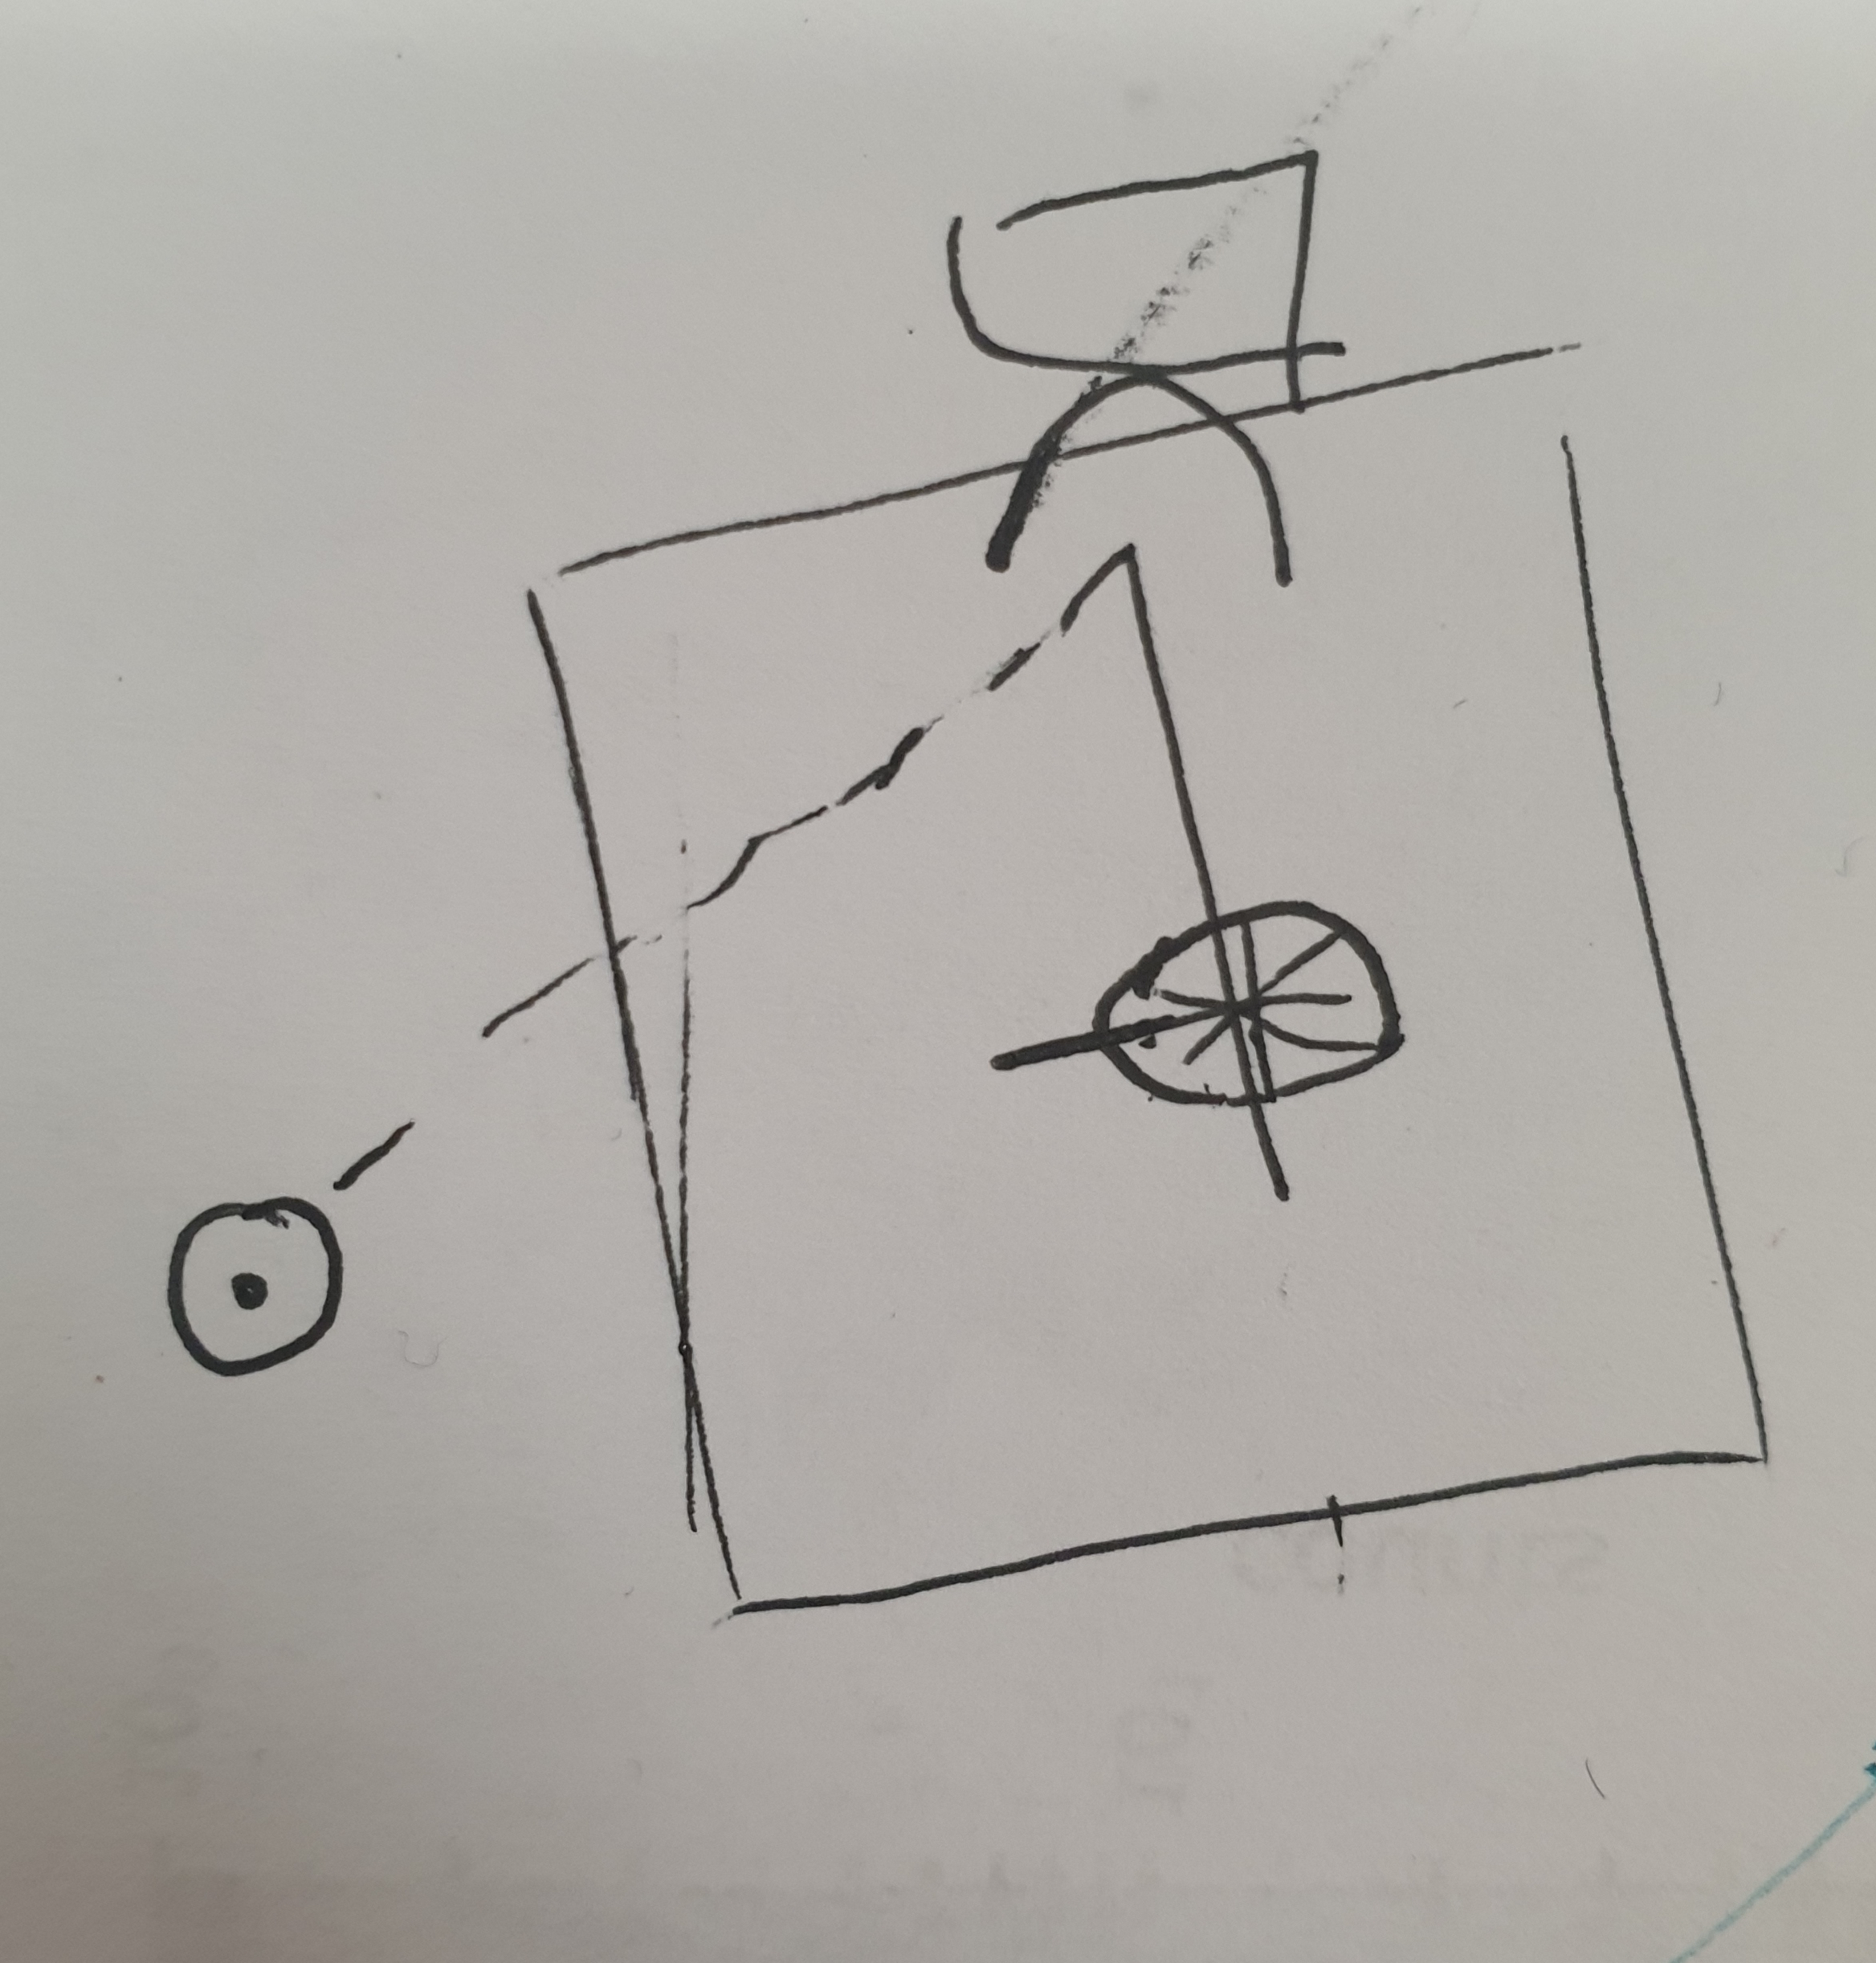
\includegraphics[width=0.5\textwidth]{Figures/dummy_sunpulse.jpg}
	\centering
	\caption{todo. Schemazeichnung Sunpulser-Problem}
	\label{fig:sp}
\end{figure}
%
%
%
\subsection{Skymaps}
\begin{figure}[h]
	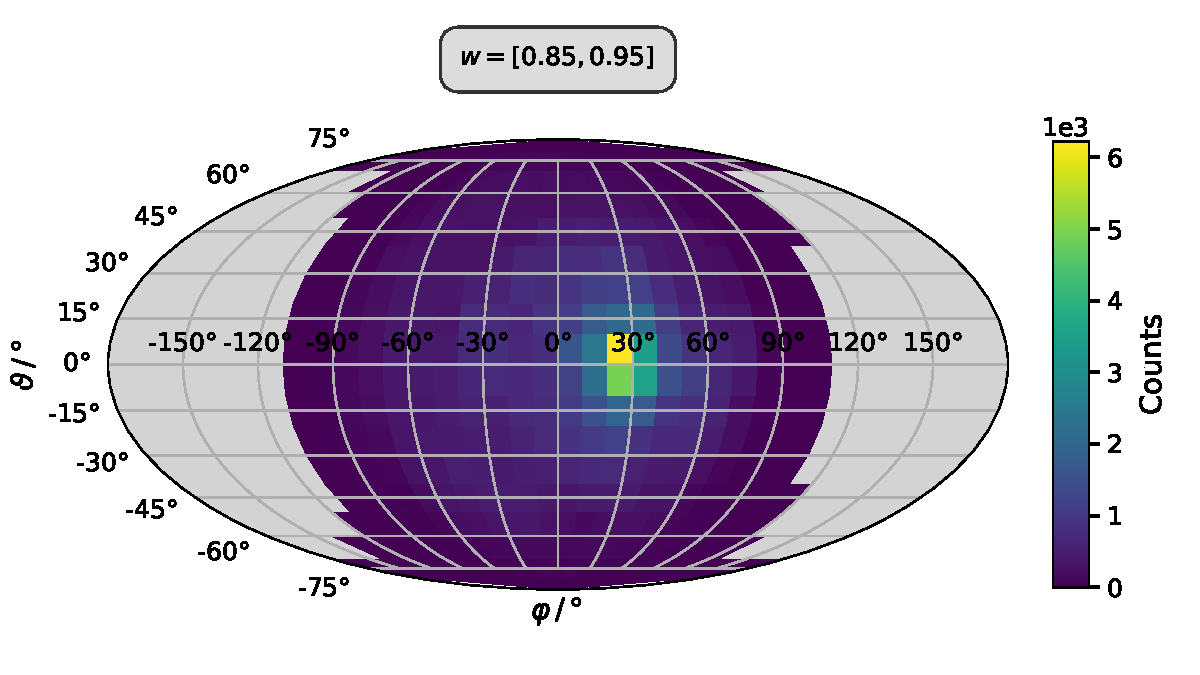
\includegraphics[width=1\textwidth]{Figures/sky_counts.pdf}
	\centering
	\caption{todo}
	\label{fig:todo}
\end{figure}
\begin{figure}[h]
	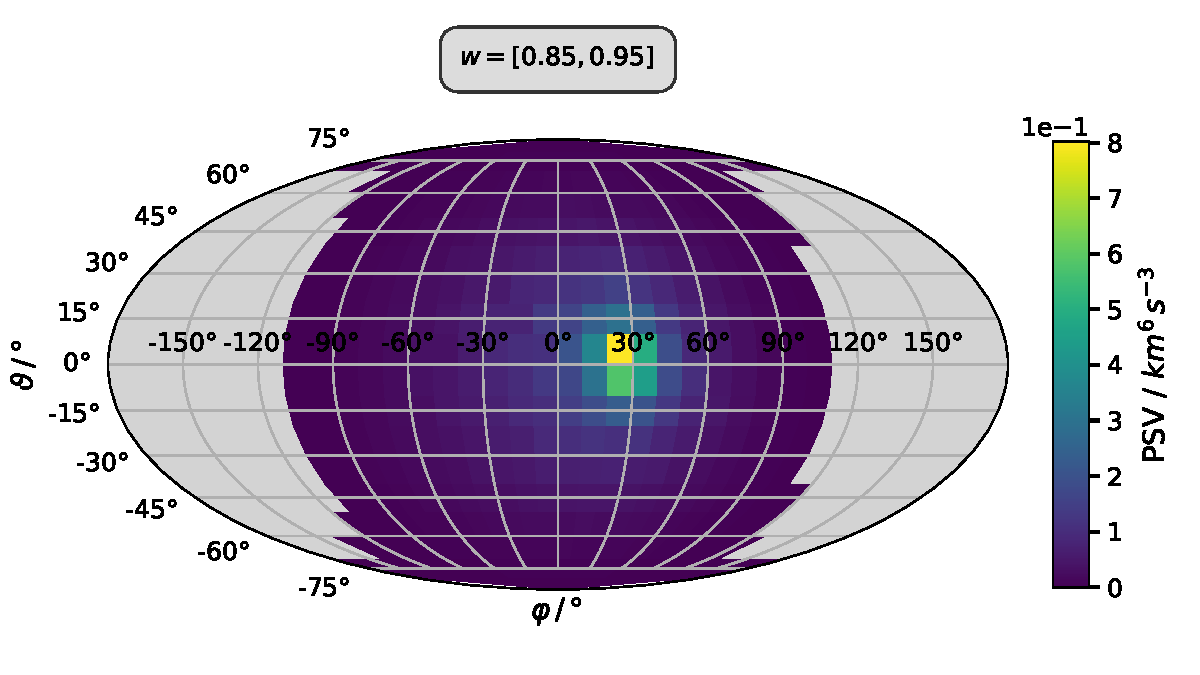
\includegraphics[width=1\textwidth]{Figures/sky_norm.pdf}
	\centering
	\caption{todo}
	\label{fig:todo}
\end{figure}
\begin{figure}[h]
	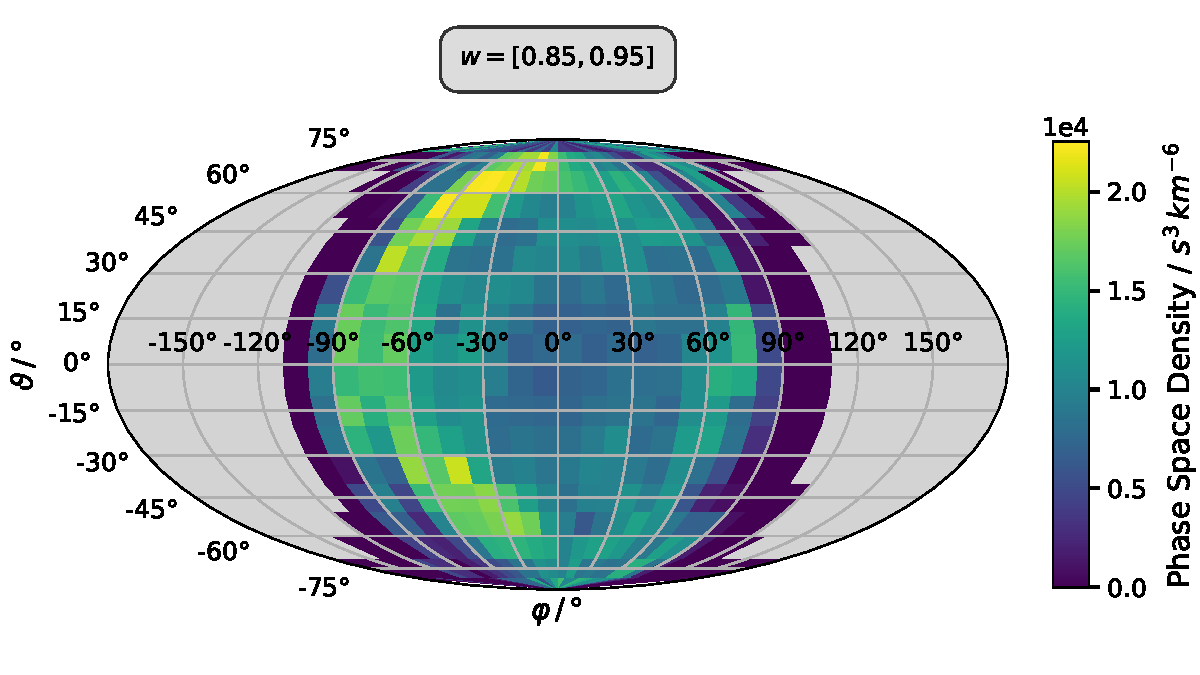
\includegraphics[width=1\textwidth]{Figures/sky_ps.pdf}
	\centering
	\caption{todo}
	\label{fig:todo}
\end{figure}
%
%
%
\subsection{1D}

\section{Outlook}
\begin{itemize}
	\item Efficiency müsste genau bestimmt werden: Dabei berücksichtigen, welcher Anteil unter den Threshold wandert. Evtl. überschätzen wir die Eff., wenn wir die interpolierten Werte von ACE/SWICS nehmen.
	\item B-Feld-spezifische Untersuchung: Torus
	\item Radialabhängigkeit: adiabatic Cooling, PA-Scattering
	\item Sonnenwindanalyse: Ist zu breit. In Richtung Spin-Achse könnte man aber über die Schalen analysieren (Lars fragen: radial?)
	
\end{itemize}





\section{Loose Ends}
\begin{itemize}
	\item andere Daten: B, vsw (Swoops: als vsw wird Protonengeschw. genommen. Ist das überhaupt richtig, ist das der Referenzframe? Und Annahme, dass vsw rein radial ist)
	\item Die Sache mit dem BRW ab 2003
	\item Englisch: Relativpronomen, Kommasetzung, British/American
	\item $\mathrm{He^{+}}$ einheitlich, mathrm
	\item Tempus?
	\item kursiv / nicht kursiv wie war das nochmal
	\item spinrate drin?
\end{itemize}
